\documentclass[12pt]{article}
\usepackage[portuguese]{babel}
\usepackage[utf8]{inputenc}
\usepackage[usenames,dvipsnames]{color}
\usepackage{setspace}
\usepackage{amsmath}
\usepackage{amsfonts}
\usepackage{amssymb}
\usepackage{mathtools}
\usepackage[top=3cm, bottom=2cm, left=3cm, right=2cm]{geometry}
\usepackage{tikz}
\usepackage{indentfirst}
\usepackage{textcomp}
\usepackage[font={small,it}]{caption}
\title{Relatorio IC}

% packages added by Marcelo
%
\usepackage{lscape}    % for landscape pages
\usepackage{hyperref}  % to allow hyperlinks
\usepackage{booktabs}  % nicer table borders
\usepackage{subfigure} % add subfigures

\newcommand{\foreignword}[1]{\textit{#1}}
\newcommand{\toolname}[1]{\textit{#1}}
%\newcommand{\fieldR}{\mathbb{R}}
\newcommand{\powerset}{\mathcal{P}}
%\newcommand{\probability}{\mathbb{P}}
%\newcommand{\expectation}{\mathbb{E}}
\newcommand{\algname}[1]{\texttt{#1}}
\newcommand{\langname}[1]{\texttt{#1}}
%\newcommand{\varname}[1]{\texttt{#1}}
%\newcommand{\floor}[1]{\lfloor #1 \rfloor}
%\newcommand{\ceil}[1]{\lceil #1 \rceil}
%\newcommand{\mathsc}[1]{{\normalfont\textsc{#1}}}
\newcommand{\forest}{\mathcal{F}}
\newcommand{\pfsnode}[1]{\mathbf #1}
\newcommand{\species}[1]{\textit{#1}}
\newcommand{\gender}[1]{\textit{#1}}

\graphicspath{{./img/}} 

\setstretch{1.5}

\begin{document}

% FAPESP demands the usage of double spacing
%
\doublespacing

\begin{titlepage}
    \vfill 
    \begin{center}
        {\Large Relatório Científico Final -- Iniciação Científica\\
         \bigskip
         Processo FAPESP 2016/25959-7
        }
        
        \bigskip
        \bigskip
    
        {\LARGE Projeto de algoritmos baseados em florestas de posets 
                para o problema de otimização U-curve}

        \bigskip
        \bigskip
        {\Large {\bf Beneficiário:} \href{mailto:gustavo.estrela.matos@usp.br}{Gustavo Estrela de Matos}\\ 
        
        {\bf Responsável:} \href{mailto:marcelo.reis@butantan.gov.br}{Marcelo da Silva Reis}\\

        \bigskip
        \bigskip
        \bigskip
        \bigskip
        \bigskip
        \bigskip
        \bigskip
Relatório referente aos trabalhos desenvolvidos entre 1 de maio e 31 de dezembro de 2017

        \bigskip
        \bigskip
        \bigskip
        \bigskip
        \bigskip
        \bigskip
        \bigskip

Laboratório Especial de Toxinologia Aplicada, Instituto Butantan\\
        \bigskip
        São Paulo, \today\\
        }

        \bigskip
        \bigskip

       

\end{center}
\end{titlepage}


\tableofcontents

\pagebreak



\section{Resumo do Projeto Proposto} \label{sec:resumo} % até 2 páginas
O problema U-curve é uma formulação de um problema de otimização que 
pode ser utilizado na etapa de seleção de características em 
Aprendizado de Máquina, com aplicações em desenho de modelos 
computacionais de sistemas biológicos. Não obstante, soluções propostas 
até o presente momento para atacar esse problema têm limitações do 
ponto de vista de consumo de tempo computacional e/ou de memória, o que 
implica na necessidade do desenvolvimento de novos algoritmos. Nesse 
sentido, em 2012 foi proposto o algoritmo 
\algname{Poset\--Forest\--Search} (\algname{PFS})~\cite{msreis thesis}, 
que organiza o espaço de busca em florestas de posets. Esse algoritmo 
foi implementado e testado, com resultados promissores; todavia, novos 
melhoramentos são necessários para que o \algname{PFS} se torne uma 
alternativa competitiva para resolver o problema U-curve. Neste projeto 
propomos modificações ao \algname{PFS} na escolha de caminhos de 
percorrimento da floresta de busca, e na estrutura de dados utilizada 
para armazenar este grafo, com o uso de diagramas de decisão binária 
ordenados (OBDDs)~\cite{bryant}; também propomos a criação 
de uma versão paralela e escalável do algoritmo \algname{PFS}. Além 
disso, propomos a criação de um algoritmo baseado no \algname{PFS} que 
tenha características de um algoritmo de aproximação, no qual o critério 
de aproximação da solução ótima se baseie no teorema da navalha de 
Ockham. Os algoritmos desenvolvidos serão implementados no arcabouço 
\toolname{featsel}~\cite{featsel paper} e testados com instâncias 
artificiais e também reais, com conjuntos de dados de aprendizado de 
máquina retirados do University of California Irvine (UCI) Machine 
Learning Repository.

 
\section{Atividades Realizadas}

Uma implementação do \algname{PFS}, feita por Reis, está disponível no
arcabouço \toolname{featsel}. Usamos esta implementação como base para
estudar as modificações feitas ao \algname{PFS}.

\subsection{Estudo de algoritmos baseados em florestas}
O algoritmo \algname{Poset\--Forest\--Search} (\algname{PFS}) é um 
algoritmo ótimo para resolver o problema de otimização U-Curve e serviu 
de base para a criação da maioria dos algoritmos elaborados neste 
trabalho. O \algname{PFS} é uma generalização de um outro algoritmo mais
simples, o \algname{U-curve-Branch-and-Bound} (\algname{UBB}), que é
um algoritmo \foreignword{branch-and-bound} ótimo que decompõe o espaço
de busca em uma árvore, e acha o mínimo global do problema fazendo 
ramificações e podas nesta árvore.

A árvore de busca do \algname{UBB} permite que a procura pelo mínimo 
ocorra de maneira parecida com uma busca em profundidade, que percorre
cadeias do reticulado Booleano de subconjuntos menores para maiores. 
Sempre que o custo de um subconjunto $X_i$ aumenta em comparação ao 
anterior $X_j$ no percorrimento, a hipótese de que a função de custo é 
decomponível em curvas em U garante que a subárvore que começa em $X_i$
pode ser removida do espaço de busca; chamamos este procedimento de
poda. O algoritmo \algname{UBB} tem, entretanto, uma limitação, pois
quando a função de custo do problema é monótona não-crescente, a 
condição de poda nunca é verdadeira e o espaço de busca inteiro é 
visitado, o que compromete a escalabilidade do algoritmo.

O \algname{PFS} enfrenta esta limitação ao fazer percorrimentos de
cadeias do espaço de busca em duas direções, de conjuntos menores para
maiores (como faz o \algname{UBB}) e também o contrário. Para fazer 
isso, este algoritmo decompõe o espaço de busca em duas árvores, uma 
para cada direção de percorrimento. Com a criação de duas estruturas 
para representar o mesmo espaço de busca, torna-se necessário a 
atualização de uma estrutura sempre que a outra sofrer mudanças, e isto
implica na utilização de florestas ao invés de árvores para representar
o espaço de busca no \algname{PFS}. Resumidamente, uma iteração do 
deste algoritmo deve escolher uma direção de percorrimento; fazer o 
percorrimento com poda (de maneira similar ao \algname{UBB}); e, 
finalmente, atualizar a floresta dual a que foi percorrida.


\subsection{Modificações do \algname{PFS} na escolha de raízes}
Para se fazer um percorrimento no espaço de busca, o algoritmo 
\algname{PFS} deve escolher uma direção de percorrimento, isto é, uma
das duas florestas que representam o espaço de busca, e também uma raiz
da floresta escolhida. Esta escolha é feita de maneira arbitrária, e por
conta disso, investigamos como diferentes escolhas podem afetar o 
desempenho do algoritmo.

Na implementação de Reis, a estrutura de dados utilizada para armazenar
raízes é a \toolname{map} do \langname{C++}. Escolhe-se nesta 
implementação o primeiro ou último elemento da estrutura, o que coincide
 com a primeira ou última raiz quando estas estão ordenadas 
lexicograficamente por seus vetores característicos. Em nosso trabalho, 
experimentamos duas modificações para esta escolha:
\begin{itemize}
    \item{de maneira aleatória e uniformemente provável;}
    \item{e de maneira determinística, com a raiz de maior sub-árvore
          completa. Neste caso, o tamanho da sub-árvore completa é o 
          tamanho deste grafo quando nenhuma poda foi feita.}
\end{itemize}

A justificativa para se fazer uma escolha uniforme entre as raízes é
ter um algoritmo que não possui viés na escolha de percorrimentos, assim 
podemos investigar se o viés da escolha arbitrária feita na 
implementação de Reis compromete a execução do algoritmo. Para fazer a 
implementação da escolha aleatória e 
uniforme fizemos uma pequena modificação ao código de Reis. Dado uma 
floresta $\forest = \{r_1, r_2, \dots, r_l\}$ sorteia-se um número 
pseudo-aleatório $a$ entre $1$ e $l$ e escolhe-se a raiz $r_a$ para o 
percorrimento.

A escolha de raiz com maior sub-árvore foi feita com a intuição de que
percorrimentos em árvores maiores implicariam em maiores podas e 
consequentemente menos nós visitados no espaço de busca. A decomposição
do espaço de busca em árvore feito por Reis faz com que ordenar as 
raízes por tamanho decrescente de sub-árvores completas coincida com 
uma ordenação lexicográfica da direita para a esquerda dos vetores 
característicos das raízes. Para fazer isto, basta modificar a 
ordenação feita pela estrutura \toolname{map} do \langname{C++}.

Chamamos o algoritmo que faz a escolha uniforme das raízes de 
\algname{PFS\_RAND}, e os resultados de tempo de execução e número
de chamadas da função de custo são apresentados na tabela 
\ref{tab:pfsrand_vs_pfs}. Podemos observar que esta modificação ao 
\algname{PFS} não foi benéfica, pois comparando com a implementação de 
Reis o tempo de execução médio aumentou, e o número médio de chamadas da 
função de custo continua parecido. O fato do número de chamadas da 
função de custo não ter diferenças significativas implica que esta 
escolha de raiz não trouxe mudanças a dinâmica do algoritmo original, 
logo o tempo a mais de execução veio do código que faz a escolha da 
raiz. Isto é feito com o percorrimento da estrutura de \toolname{map}, 
o que adiciona tempo linear (sobre a quantidade de raízes) a cada 
escolha de raiz.

\begin{table}
\centering
\footnotesize
\caption{Comparação entre os algoritmos \algname{PFS} e 
\algname{PFS\_RAND}. O tempo de execução do segundo é maior do que o 
primeiro enquanto a quantidade de chamadas da função custo é parecida
em ambos.} \label{tab:pfsrand_vs_pfs}
 \resizebox{\columnwidth}{!}{%
\begin{tabular}{cc c cc c cc}
\toprule
\multicolumn{2}{c}{Instância} & \phantom{} & \multicolumn{2}{c}{Tempo de execução médio (s)}  & \phantom{} & \multicolumn{2}{c}{Número médio de cálculos de custo}\\
\cline{1-2}\cline{4-5}\cline{7-8}\\
$|S|$ & $2^{|S|}$ && \algname{PFS} & \algname{PFS\_RAND} && \algname{PFS} & \algname{PFS\_RAND} \\
10 &    1024 &&  0.013 $\pm$ 0.003 & 0.014 $\pm$ 0.003 &&   590.8 $\pm$ 198.5 & 599.5 $\pm$ 177.5 \\
11 &    2048 &&  0.019 $\pm$ 0.004 & 0.022 $\pm$ 0.007 &&   1114.8 $\pm$ 331.3 & 1090.1 $\pm$ 350.3 \\
12 &    4096 &&  0.029 $\pm$ 0.008 & 0.036 $\pm$ 0.013 &&   1848.6 $\pm$ 600.8 & 1835.7 $\pm$ 683.0 \\
13 &    8192 &&  0.060 $\pm$ 0.018 & 0.090 $\pm$ 0.039 &&   4314.4 $\pm$ 1496.4 & 4201.1 $\pm$ 1580.7 \\
14 &   16384 &&  0.100 $\pm$ 0.041 & 0.191 $\pm$ 0.110 &&   7323.4 $\pm$ 3318.9 & 7333.8 $\pm$ 3161.0 \\
15 &   32768 &&  0.180 $\pm$ 0.076 & 0.453 $\pm$ 0.311 &&   12958.1 $\pm$ 5654.0 & 12807.5 $\pm$ 5753.7 \\
16 &   65536 &&  0.406 $\pm$ 0.185 & 1.715 $\pm$ 1.400 &&   27573.8 $\pm$ 12459.5 & 27036.9 $\pm$ 12687.5 \\
17 &  131072 &&  0.717 $\pm$ 0.397 & 5.416 $\pm$ 5.266 &&   48176.2 $\pm$ 26938.3 & 47852.1 $\pm$ 26427.6 \\
18 &  262144 &&  1.325 $\pm$ 0.754 & 15.890 $\pm$ 17.726 &&   84417.9 $\pm$ 48587.7 & 84025.0 $\pm$ 48882.4 \\
19 &  524288 &&  2.771 $\pm$ 1.603 & 69.600 $\pm$ 82.342 &&   167659.1 $\pm$ 99686.7 & 164612.1 $\pm$ 102018.3 \\
\bottomrule
\end{tabular}%
 }
\end{table}

Chamamos de \algname{PFS\_LEFTMOST} o algoritmo que faz a escolha da 
raiz com maior sub-árvore completa, e a 
tabela~\ref{tab:pfsleftmost_vs_pfs} mostra resultados de tempo de 
execução e número de chamadas da função de custo desta variante 
comparado a implementação de Reis. Podemos observar que esta modificação
também não foi benéfica pois, além do maior tempo de execução, o número
de chamadas da função de custo aumentou. Isto significa que o 
comportamento do algoritmo foi o contrário a intuição que motivou a 
modificação, pois mais nós do espaço de busca foram visitados.

\begin{table}
\centering
\footnotesize
\caption{Comparação entre os algoritmos \algname{PFS} e 
\algname{PFS\_LEFTMOST}. O tempo de execução e também o número de 
chamadas da função custo é maior para o \algname{PFS\_LEFTMOST}.} 
\label{tab:pfsleftmost_vs_pfs}
 \resizebox{\columnwidth}{!}{%
\begin{tabular}{cc c cc c cc}
\toprule
\multicolumn{2}{c}{Instância} & \phantom{} & \multicolumn{2}{c}{Tempo de execução médio (s)}  & \phantom{} & \multicolumn{2}{c}{Número médio de cálculos de custo}\\
\cline{1-2}\cline{4-5}\cline{7-8}\\
$|S|$ & $2^{|S|}$ && \algname{PFS} & \algname{PFS\_LEFTMOST} && \algname{PFS} & \algname{PFS\_LEFTMOST} \\
10 &    1024 &&  0.013 $\pm$ 0.002 & 0.023 $\pm$ 0.004 &&  606.1 $\pm$ 133.5 & 665.0 $\pm$ 165.8 \\
11 &    2048 &&  0.020 $\pm$ 0.004 & 0.042 $\pm$ 0.010 &&  1122.1 $\pm$ 351.2 & 1316.6 $\pm$ 382.2 \\
12 &    4096 &&  0.032 $\pm$ 0.008 & 0.078 $\pm$ 0.024 &&  2183.7 $\pm$ 733.2 & 2515.8 $\pm$ 871.3 \\
13 &    8192 &&  0.054 $\pm$ 0.017 & 0.160 $\pm$ 0.061 &&  3887.7 $\pm$ 1389.9 & 4716.8 $\pm$ 1777.8 \\
14 &   16384 &&  0.107 $\pm$ 0.034 & 0.345 $\pm$ 0.133 &&  7851.2 $\pm$ 2793.0 & 9506.8 $\pm$ 3673.9 \\
15 &   32768 &&  0.196 $\pm$ 0.085 & 0.672 $\pm$ 0.274 &&  13780.3 $\pm$ 6049.9 & 17071.6 $\pm$ 7005.1 \\
16 &   65536 &&  0.348 $\pm$ 0.189 & 1.271 $\pm$ 0.661 &&  24106.5 $\pm$ 13159.9 & 30055.6 $\pm$ 15363.6 \\
17 &  131072 &&  0.785 $\pm$ 0.361 & 3.137 $\pm$ 1.476 &&  52369.0 $\pm$ 24751.2 & 67585.6 $\pm$ 30978.4 \\
18 &  262144 &&  1.445 $\pm$ 0.657 & 6.146 $\pm$ 3.032 &&  92095.9 $\pm$ 42566.6 & 120635.7 $\pm$ 58039.0 \\
19 &  524288 &&  3.298 $\pm$ 1.883 & 13.881 $\pm$ 7.595 &&  199151.0 $\pm$ 112167.8 & 256078.6 $\pm$ 135958.4 \\
%20 & 1048576 &&  6.141 $\pm$ 3.728 & 28.733 $\pm$ 18.120 &&  356259.2 $\pm$ 218253.1 & 465255.8 $\pm$ 276843.3 \\
%21 & 2097152 &&  10.817 $\pm$ 7.714 & 52.374 $\pm$ 38.565 &&  608984.4 $\pm$ 432151.7 & 801620.2 $\pm$ 561000.7 \\
\bottomrule 
\end{tabular}%
 }
\end{table}

\subsection{Mudificação do \algname{PFS} no armazenamento de raízes}
A quantidade de raízes durante a execução do \algname{PFS} pode ser 
grande, e por isso a estrutura utilizada para o seu armazenamento deve
ser eficiente para operações como inserções, remoções e consultas. 
Motivados por resultados de um trabalho de iniciação científica 
anterior (FAPESP processo \#2014/23564-0), experimentamos o uso de
diagramas de decisão binária ordenados (OBDDs) para o armazenamento
de raízes.

A estrutura de OBDD é um diagrama capaz de representar funções Booleanas
$f: \{0, 1\}^n \to \{0, 1\}$. Para utilizarmos esta estrutura no 
armazenamento de raízes, criamos uma OBDD que representa a função que 
mapeia para valores $1$ os subconjuntos que são raízes da floresta
e para $0$ os demais. Para de fato armazenar as raízes tivemos que 
modificar a estrutura usual de OBDD, então ao invés de usar folhas com 
valores $0$ ou $1$, usamos folhas que armazenam nós do espaço de busca
ou um ponteiro nulo. A figura~\ref{fig:pfs:obdd} mostra um exemplo de 
floresta do espaço de busca e a correspondente representação em nossa 
estrutura de OBDD. 

\begin{figure}[]
  \centering 
  \begin{tabular}{c c}
    \subfigure {\scalebox{.7}{
     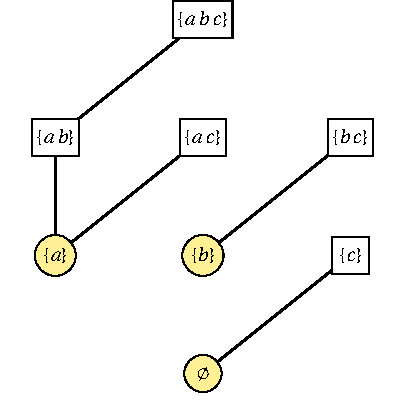
\includegraphics[clip=true]{pfs/obdd/lattice.pdf}}
     \label{fig:pfs:obdd:A} }
      & 
      \subfigure {\scalebox{.9}{
    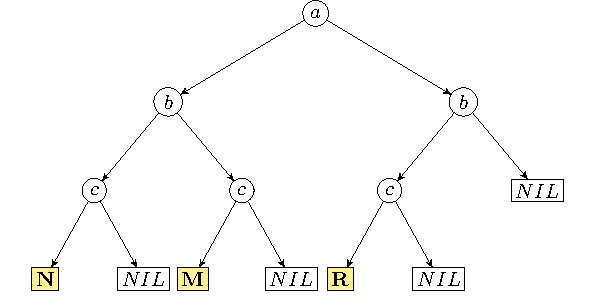
\includegraphics[clip=true]{pfs/obdd/obdd.pdf}}
        \label{fig:pfs:obdd:B} }
  \end{tabular}
  \caption{Exemplo de OBDD que representa uma floresta do 
    \algname{PFS}. Esta OBDD contém os nós $\pfsnode{N}$, $\pfsnode{M}$
    e $\pfsnode{R}$, que representam respectivamente os subconjuntos
    $000$, $010$ e $100$. As folhas $NIL$ indicam que os subconjuntos 
    de tal caminho na OBDD não são raízes na floresta, como por exemplo 
    os subconjuntos $11X$}
  \label{fig:pfs:obdd}
\end{figure}

Como a estrutura de dados que armazena as raízes foi modificada, é 
necessário definir o abordagem para escolha de raiz na etapa de 
percorrimento. Utilizamos então a abordagem de escolha aleatória e 
uniforme, pois esta mostrou uma dinâmica similar a implementação de
Reis.

Chamamos o algoritmo que usa OBDDs para armazenamento de raízes de 
\algname{OPFS}. A tabela~\ref{tab:opfs_vs_pfs} mostra uma comparação de
tempo de execução e número de cálculos da função de custo entre o 
algoritmo original e esta modificação. Observamos que o número de 
chamadas da função custo é similar enquanto o tempo de execução é maior
para o algoritmo \algname{OPFS}, portanto esta modificação não trouxe 
melhoras ao algoritmo \algname{PFS}.

\begin{table}
\centering
\footnotesize
\caption{Comparação entre os algoritmos \algname{PFS} e \algname{OPFS}. 
O número de chamadas médio da função custo é parecido enquanto o tempo
de execução é maior para o \algname{OBDD}.}
\label{tab:opfs_vs_pfs}
\begin{tabular}{cc c cc c cc}
\toprule
\multicolumn{2}{c}{Instância} & \phantom{} & \multicolumn{2}{c}{Tempo de execução médio (s)}  & \phantom{} & \multicolumn{2}{c}{Número médio de cálculos de custo}\\
\cline{1-2}\cline{4-5}\cline{7-8}\\
$|S|$ & $2^{|S|}$ && \algname{PFS} & \algname{OPFS} && \algname{PFS} & \algname{OPFS} \\
10 &    1024 &&  0.013 $\pm$ 0.003 & 0.018 $\pm$ 0.003 &&  598.0 $\pm$ 192.8 & 635.5 $\pm$ 171.9 \\
11 &    2048 &&  0.020 $\pm$ 0.004 & 0.029 $\pm$ 0.007 &&  1152.1 $\pm$ 314.7 & 1117.9 $\pm$ 336.4 \\
12 &    4096 &&  0.031 $\pm$ 0.010 & 0.049 $\pm$ 0.013 &&  2024.1 $\pm$ 751.6 & 2048.2 $\pm$ 700.9 \\
13 &    8192 &&  0.057 $\pm$ 0.017 & 0.097 $\pm$ 0.033 &&  3996.3 $\pm$ 1431.6 & 3973.4 $\pm$ 1462.6 \\
14 &   16384 &&  0.094 $\pm$ 0.038 & 0.171 $\pm$ 0.063 &&  6634.8 $\pm$ 2944.0 & 6906.5 $\pm$ 2786.5 \\
15 &   32768 &&  0.182 $\pm$ 0.079 & 0.323 $\pm$ 0.156 &&  13140.1 $\pm$ 6020.6 & 12711.2 $\pm$ 6319.7 \\
16 &   65536 &&  0.370 $\pm$ 0.169 & 0.660 $\pm$ 0.314 &&  25658.2 $\pm$ 11606.7 & 25303.4 $\pm$ 12169.5 \\
17 &  131072 &&  0.819 $\pm$ 0.370 & 1.480 $\pm$ 0.665 &&  53344.9 $\pm$ 24350.4 & 53217.2 $\pm$ 24154.5 \\
18 &  262144 &&  1.515 $\pm$ 0.905 & 2.736 $\pm$ 1.626 &&  94677.6 $\pm$ 54496.3 & 94079.4 $\pm$ 55435.6 \\
19 &  524288 &&  2.612 $\pm$ 1.869 & 4.818 $\pm$ 3.355 &&  156150.5 $\pm$ 107369.8 & 156021.8 $\pm$ 107516.8 \\
20 & 1048576 &&  6.085 $\pm$ 3.900 & 11.550 $\pm$ 7.661 &&  344144.1 $\pm$ 212627.1 & 343229.2 $\pm$ 212624.4 \\
% 21 & 2097152 &&  11.416 $\pm$ 8.296 & 21.818 $\pm$ 16.269 &&  616936.2 $\pm$ 436491.2 & 613526.2 $\pm$ 438580.0 \\
% 22 & 4194304 &&  19.950 $\pm$ 17.799 & 42.112 $\pm$ 45.109 &&  960842.2 $\pm$ 785137.2 & 959905.4 $\pm$ 783257.3 \\
% 23 & 8388608 &&  42.792 $\pm$ 35.622 & 87.262 $\pm$ 90.579 &&  2053472.4 $\pm$ 1690882.1 & 2060184.5 $\pm$ 1682011.0 \\
% 24 & 16777216 &&  85.646 $\pm$ 79.186 & 149.567 $\pm$ 108.104 &&  4080290.8 $\pm$ 3166258.4 & 4100480.6 $\pm$ 3141423.9 \\
\bottomrule 
\end{tabular}%
\end{table}


\subsection{Paralelização do \algname{PFS}}
A decomposição do espaço de busca em uma floresta feita pelo algoritmo
\algname{PFS} separa tal espaço em partes disjuntas que são árvores.
Estruturas disjuntas como estas podem ser percorridas de maneira 
paralela sem ou com poucas interferências entre linhas de processamento,
portanto a paralelização do algoritmo \algname{PFS} pode trazer ganhos 
em tempo de execução. Desta maneira, paralelizamos este algoritmo, e 
para isso utilizamos a biblioteca \toolname{OpenMP}.

Entretanto, apesar da etapa de percorrimento das árvores ser quase 
independente entre linhas de processamento paralelas, a etapa de 
atualização da floresta dual a que foi percorrida é dependente. Além
de possuir seções críticas, em que apenas uma linha de processamento 
pode avançar de cada vez, a atualização da floresta dual pode ter
condições de corrida, isto é, o resultado da atualização pode depender
da ordem em que as linhas de processamento avançam no código. Condições
de corrida não tratadas podem inclusive levar a inconsistências na
representação do espaço de busca.

Este algoritmo paralelo foi chamado de \algname{PPFS}. Testamos o 
desempenho deste algoritmo comparado ao \algname{PFS} e os resultados
são apresentados na tabela~\ref{tab:ppfs_vs_pfs}. Podemos notar que o
tempo de execução do algoritmo paralelo é pior do que a versão original,
portanto o trabalho adicional de controle de linhas de processamento
não é recompensado pelo ganho de tempo de processamento paralelo. Isto
aconteceu porque a etapa de ramificação, que pode ser feita em paralelo
sem grandes dificuldades, é curta em relação a etapa de atualização de
floresta dual, que possui diversas seções críticas e também um código
adicional para controle de condições de corrida.


\begin{table}
\centering
\footnotesize
\caption{Comparação entre os algoritmos \algname{PFS} e \algname{PPFS}.
O algoritmo \algname{PPFS} apresenta um número similar de média de 
chamadas da função custo ao \algname{PFS}, mas possui tempo de execução 
médio maior.}
\label{tab:ppfs_vs_pfs}
% \resizebox{\columnwidth}{!}{%
\begin{tabular}{cc c cc c cc}
\toprule
\multicolumn{2}{c}{Instância} & \phantom{} & \multicolumn{2}{c}{Tempo de execução médio (s)} & \phantom{} & \multicolumn{2}{c}{Número médio de cálculos de custo} \\
\cline{1-2}\cline{4-5}\cline{7-8}\\
$|S|$ & $2^{|S|}$ && \algname{PFS} & \algname{PPFS} && \algname{PFS} & \algname{PPFS} \\
 % 1 &       2 && 0.005 $\pm$ 0.004 & 0.028 $\pm$ 0.006 &&  2.0 $\pm$  0.0 &  2.0 $\pm$  0.0 \\
 % 2 &       4 && 0.004 $\pm$ 0.000 & 0.038 $\pm$ 0.008 &&  3.9 $\pm$  0.3 &  3.9 $\pm$  0.3 \\
 % 3 &       8 && 0.004 $\pm$ 0.000 & 0.039 $\pm$ 0.007 &&  7.0 $\pm$  1.2 &  7.0 $\pm$  1.2 \\
 % 4 &      16 && 0.004 $\pm$ 0.000 & 0.047 $\pm$ 0.008 && 12.8 $\pm$  3.0 & 13.2 $\pm$  3.3 \\
 % 5 &      32 && 0.005 $\pm$ 0.000 & 0.058 $\pm$ 0.009 && 26.8 $\pm$  4.5 & 26.9 $\pm$  3.0 \\
 % 6 &      64 && 0.005 $\pm$ 0.000 & 0.061 $\pm$ 0.010 && 52.7 $\pm$  7.3 & 50.5 $\pm$  6.4 \\
 % 7 &     128 && 0.005 $\pm$ 0.000 & 0.070 $\pm$ 0.013 && 87.3 $\pm$ 20.5 & 82.8 $\pm$ 23.5 \\
 % 8 &     256 && 0.006 $\pm$ 0.000 & 0.079 $\pm$ 0.013 && 177.0 $\pm$ 32.1 & 171.2 $\pm$ 36.2 \\
 % 9 &     512 && 0.008 $\pm$ 0.001 & 0.104 $\pm$ 0.021 && 333.8 $\pm$ 93.9 & 344.5 $\pm$ 95.2 \\
10 &    1024 && 0.011 $\pm$ 0.001 & 0.146 $\pm$ 0.027 && 643.6 $\pm$ 133.0 & 626.5 $\pm$ 151.1 \\
11 &    2048 && 0.017 $\pm$ 0.004 & 0.227 $\pm$ 0.062 && 1151.0 $\pm$ 359.7 & 1135.6 $\pm$ 381.1 \\
12 &    4096 && 0.029 $\pm$ 0.007 & 0.385 $\pm$ 0.113 && 2173.1 $\pm$ 652.5 & 2139.2 $\pm$ 710.3 \\
13 &    8192 && 0.049 $\pm$ 0.015 & 0.640 $\pm$ 0.237 && 3839.8 $\pm$ 1376.6 & 3743.5 $\pm$ 1532.9 \\
14 &   16384 && 0.104 $\pm$ 0.037 & 1.337 $\pm$ 0.513 && 8175.9 $\pm$ 3037.4 & 8026.4 $\pm$ 3303.7 \\
15 &   32768 && 0.163 $\pm$ 0.078 & 2.010 $\pm$ 1.096 && 12459.6 $\pm$ 6164.5 & 12062.2 $\pm$ 6897.2 \\
16 &   65536 && 0.360 $\pm$ 0.163 & 4.483 $\pm$ 2.030 && 27027.3 $\pm$ 12397.0 & 26835.7 $\pm$ 12446.9 \\
17 &  131072 && 0.664 $\pm$ 0.362 & 8.072 $\pm$ 4.370 && 48001.9 $\pm$ 26149.2 & 48093.4 $\pm$ 26233.2 \\
18 &  262144 && 1.250 $\pm$ 0.690 & 14.341 $\pm$ 8.062 && 85880.9 $\pm$ 47950.8 & 86050.8 $\pm$ 49186.8 \\
19 &  524288 && 2.936 $\pm$ 1.629 & 34.639 $\pm$ 19.074 && 198503.0 $\pm$ 108116.1 & 197832.5 $\pm$ 110659.6 \\
20 & 1048576 && 5.024 $\pm$ 3.097 & 61.038 $\pm$ 38.250 && 321495.8 $\pm$ 198004.3 & 318507.0 $\pm$ 199354.3 \\
% 21 & 2097152 && 11.997 $\pm$ 7.637 & 144.610 $\pm$ 89.521 && 754636.3 $\pm$ 478683.6 & 759129.7 $\pm$ 472831.1 \\
\bottomrule
\end{tabular}
% }
\end{table}


\subsection{Elaboração do \algname{UBB-PFS}}
Visto que a paralelização do \algname{PFS} não teve bons resultados 
devido o entrelace de linhas de processamento na atualização da floresta 
dual, criamos um novo algoritmo paralelo em que as linhas de execução
interferem minimamente uma nas outras. Este algoritmo particiona o 
espaço de busca e resolve cada parte de maneira paralela e independente
como um sub-problema do problema original. Chamamos este algoritmo de 
\algname{UBB-PFS} porque ele possui duas etapas em que procedimentos 
similares ao \algname{UBB} e o \algname{PFS} ocorrem. 

Na primeira etapa, percorre-se o reticulado de maneira idêntica a que 
se faz no algoritmo \algname{UBB}, ou seja, com uma busca em
profundidade. A cada iteração deste percorrimento, a pilha de busca em 
profundidade contém nós que são raízes de sub-árvores completas do
espaço de busca. Portanto, a cada iteração da primeira etapa, o espaço
de busca está particionado nas seguintes partes:
\begin{itemize}
    \item{Subconjuntos visitados na primeira etapa: estes subconjuntos
        entraram na pilha de busca de profundidade, foram visitados e 
        foram removidos da pilha. O custo de todos estes subconjuntos 
        foram calculados.}
    \item{Subconjuntos não visitados na primeira etapa: estes elementos
        estão contidos em uma das sub-árvores com raiz na pilha de
        busca em profundidade. Note este conjunto é particionado por
        estas sub-árvores.}
\end{itemize}

Desta maneira, a cada iteração da primeira etapa, podemos encontrar a
solução do problema ao encontrar a melhor solução entre o mínimo dos
elementos visitados e o mínimo de cada uma das partes que são 
sub-árvores. Determinar o mínimo dos elementos visitados é fácil, pois
o custo destes elementos já foi calculado no percorrimento, já
para determinar o mínimo dos elementos não visitados é necessário 
resolver sub-problemas do problema original, o que é feito na segunda
etapa do \algname{UBB-PFS}.

A decomposição do espaço de busca em uma árvore feita pelo algoritmo
\algname{UBB} permite que cada sub-árvore do espaço de busca seja
representada também por um reticulado Booleano completo. Desta maneira,
é possível transformar o problema de encontrar o mínimo local  de uma 
sub-árvore em um problema de seleção de características. A segunda etapa 
do \algname{UBB-PFS} é então responsável por mapear cada uma das 
sub-árvores não percorridas do espaço de busca em um problema auxiliar
de seleção de características e resolvê-los em paralelo com chamadas
do algoritmo \algname{PFS}. Como estes sub-problemas são independentes,
as chamadas em paralelo devem ter pouco ou nenhum entrelace, o que deve
trazer a melhora de desempenho que não foi possível com a simples 
paralelização do \algname{PFS}.

Entretanto, ainda é necessário definir em que momento o algoritmo deve
passar da primeira para a segunda etapa. A princípio, esta transição
pode ocorrer em qualquer fim de iteração da busca em profundidade, 
entretanto fazer esta transição prematuramente pode implicar em um 
particionamento grosso do espaço de busca, com poucas raízes na pilha
de busca em profundidade; por outro lado, quanto mais tarde fizermos 
esta transição, menor será o trabalho realizado em paralelo, já que a
primeira etapa  é feita sempre de maneira serial. Definimos em nossa 
implementação que a transição deve ocorrer sempre que o número de 
sub-árvores for maior do que o número de núcleos de processamento do 
computador ou quando o número de iterações da primeira etapa for maior
do que duas vezes a quantidade de características do problema.

A tabela~\ref{tab:ubbpfs_vs_ubb_vs_pfs_time} mostra a comparação de 
tempo de execução entre os algoritmos \algname{UBB}, \algname{PFS} e
\algname{UBB-PFS}. Apesar do \algname{UBB} possuir limitações quando
a função é monotônica não-crescente, este é o algoritmo mais rápido
no caso médio, seguido pelo \algname{UBB-PFS}, e o \algname{PFS} é o 
mais lento. A tabela~\ref{tab:ubbpfs_vs_ubb_vs_pfs_computed_nodes} 
mostra a comparação de número de chamadas da função custo, e podemos
observar que o \algname{PFS} tem o menor número, seguido pelo 
\algname{UBB-PFS} e o \algname{UBB}, que possui maior número de 
chamadas.

\begin{table}
\centering
\footnotesize
\caption{Comparação de tempo médio de execução entre os algoritmos
\algname{UBB}, \algname{PFS} e \algname{UBB-PFS}. Podemos observar que
o \algname{PFS} foi o mais lento enquanto o \algname{UBB} foi o mais
rápido e o \algname{UBB-PFS} teve desempenho itermediário para estas
instâncias.}
\label{tab:ubbpfs_vs_ubb_vs_pfs_time}
% \resizebox{\columnwidth}{!}{%
\begin{tabular}{cc c ccc}
\toprule
\multicolumn{2}{c}{Instância} & \phantom{} & \multicolumn{3}{c}{Tempo de execução médio (s)}\\
\cline{1-2}\cline{4-6}\\
$|S|$ & $2^{|S|}$ && \algname{UBB} & \algname{PFS} & \algname{UBB-PFS}  \\
10 &    1024 &&  0.006 $\pm$ 0.001 & 0.011 $\pm$ 0.002 & 0.023 $\pm$ 0.004 \\
11 &    2048 &&  0.007 $\pm$ 0.001 & 0.017 $\pm$ 0.004 & 0.026 $\pm$ 0.004 \\
12 &    4096 &&  0.010 $\pm$ 0.003 & 0.029 $\pm$ 0.009 & 0.034 $\pm$ 0.006 \\
13 &    8192 &&  0.013 $\pm$ 0.006 & 0.047 $\pm$ 0.016 & 0.044 $\pm$ 0.011 \\
14 &   16384 &&  0.024 $\pm$ 0.013 & 0.094 $\pm$ 0.034 & 0.068 $\pm$ 0.023 \\
15 &   32768 &&  0.043 $\pm$ 0.026 & 0.186 $\pm$ 0.074 & 0.113 $\pm$ 0.042 \\
16 &   65536 &&  0.083 $\pm$ 0.060 & 0.339 $\pm$ 0.168 & 0.187 $\pm$ 0.082 \\
17 &  131072 &&  0.161 $\pm$ 0.122 & 0.650 $\pm$ 0.347 & 0.326 $\pm$ 0.175 \\
18 &  262144 &&  0.321 $\pm$ 0.233 & 1.482 $\pm$ 0.768 & 0.703 $\pm$ 0.380 \\
19 &  524288 &&  0.620 $\pm$ 0.447 & 2.711 $\pm$ 1.562 & 1.309 $\pm$ 0.729 \\
20 & 1048576 &&  1.312 $\pm$ 0.970 & 5.007 $\pm$ 3.302 & 2.478 $\pm$ 1.547 \\
21 & 2097152 &&  2.494 $\pm$ 1.893 & 11.125 $\pm$ 6.749 & 5.458 $\pm$ 3.294 \\
22 & 4194304 &&  4.589 $\pm$ 4.122 & 19.085 $\pm$ 15.147 & 8.832 $\pm$ 6.846 \\
23 & 8388608 &&  12.228 $\pm$ 7.922 & 40.323 $\pm$ 29.649 & 18.891 $\pm$ 12.786 \\
24 & 16777216 &&  24.273 $\pm$ 16.277 & 113.332 $\pm$ 76.688 & 67.178 $\pm$ 46.516 \\
\bottomrule
\end{tabular}
% }
\end{table}


\begin{table}
\centering
\footnotesize
\caption{Comparação sobre o número de chamadas de função custo entre
os algoritmos \algname{UBB}, \algname{PFS} e \algname{UBB-PFS}. Vemos
nesta tabela que o número de nós computados pelo \algname{UBB} é o maior
enquanto o do \algname{PFS} é o menor; o \algname{UBB-PFS} tem 
desempenho intermediário, porém próximo ao do \algname{PFS}.}
\label{tab:ubbpfs_vs_ubb_vs_pfs_computed_nodes}
% \resizebox{\columnwidth}{!}{%
\begin{tabular}{cc c ccc}
\toprule
\multicolumn{2}{c}{Instância} & \phantom{} & \multicolumn{3}{c}{Número médio de cálculos de custo}\\
\cline{1-2}\cline{4-6} \\
$|S|$ & $2^{|S|}$ && \algname{UBB} & \algname{PFS} & \algname{UBB-PFS}  \\
10 &    1024  && 699.4 $\pm$ 361.3 & 611.3 $\pm$ 178.8 & 634.7 $\pm$ 209.8 \\
11 &    2048  && 1217.2 $\pm$ 747.1 & 1145.4 $\pm$ 358.9 & 1178.8 $\pm$ 484.1 \\
12 &    4096  && 2898.0 $\pm$ 1380.4 & 2103.1 $\pm$ 793.6 & 2363.0 $\pm$ 760.4 \\
13 &    8192  && 4422.6 $\pm$ 3293.8 & 3650.9 $\pm$ 1371.9 & 3934.4 $\pm$ 1487.7 \\
14 &   16384  && 10089.4 $\pm$ 6452.1 & 7536.3 $\pm$ 2926.1 & 8012.2 $\pm$ 3387.4 \\
15 &   32768  && 19097.5 $\pm$ 12793.8 & 14546.5 $\pm$ 6081.0 & 15299.2 $\pm$ 6598.4 \\
16 &   65536  && 37663.1 $\pm$ 28321.2 & 25744.0 $\pm$ 12795.4 & 27028.4 $\pm$ 13031.9 \\
17 &  131072  && 73373.3 $\pm$ 55994.3 & 46808.9 $\pm$ 24533.5 & 49348.6 $\pm$ 24556.7 \\
18 &  262144  && 150035.2 $\pm$ 108299.3 & 103166.6 $\pm$ 52464.7 & 105306.4 $\pm$ 53472.0 \\
19 &  524288  && 292561.2 $\pm$ 210771.2 & 183125.7 $\pm$ 104965.4 & 189545.7 $\pm$ 102145.9 \\
20 & 1048576  && 617049.5 $\pm$ 450468.2 & 323097.4 $\pm$ 213634.3 & 340694.2 $\pm$ 202389.6 \\
21 & 2097152  && 1172641.6 $\pm$ 879148.5 & 691991.3 $\pm$ 413262.9 & 704790.2 $\pm$ 407143.8 \\
22 & 4194304  && 2099973.2 $\pm$ 1863285.8 & 1133395.1 $\pm$ 874492.0 & 1156564.2 $\pm$ 862152.0 \\
23 & 8388608  && 5435778.8 $\pm$ 3468245.3 & 2276694.5 $\pm$ 1621342.2 & 2345648.2 $\pm$ 1558258.5 \\
24 & 16777216 && 10146842.9 $\pm$ 6673018.3 & 5527504.2 $\pm$ 3413432.3 & 5609052.7 $\pm$ 3337059.1 \\
\bottomrule
\end{tabular}
% }
\end{table}
Estes resultados mostram que o desempenho do \algname{UBB-PFS} é 
intermediário entre o \algname{UBB} e \algname{PFS} para dois parâmetros
diferentes de qualidade. Portanto, podemos considerar o 
\algname{UBB-PFS} uma opção competitiva para problemas de seleção de 
características.


\subsection{Elaboração do \algname{Parallel-U-Curve-Search}}
Apesar do algoritmo \algname{UBB-PFS} ser uma opção competitiva para o
problema de seleção de características, este algoritmo possui pontos
que poderiam ser explorados para se obter uma melhor paralelização. 
Entre estes pontos, podemos citar a divisão de trabalho do algoritmo,
que é arbitrária e depende da busca em profundidade, 
o que não é ideal, pois uma boa paralelização deve tentar dividir o 
trabalho de maneira igual entre os núcleos dos processadores; além 
disso, a escolha do momento de finalização da primeira etapa para a 
segunda também é arbitrária; por último, a criação de sub-problemas de
seleção de características indica que este algoritmo poderia ser
recursivo.

O cronograma da proposta deste trabalho inclui a elaboração de um 
algoritmo de aproximação para o problema U-curve, porém optamos em 
continuar estudando algoritmos paralelos para o problema U-curve, o que 
nos levou a construção do algoritmo 
\algname{Parallel\--U-curve\--Search} (\algname{PUCS}). Ao contrário do
\algname{UBB-PFS} que é uma adaptação paralela de algoritmos já 
existentes, o \algname{PUCS} é um algoritmo que foi criado com o intuito
de ser paralelo, usando um esquema de divisão e conquista.

Assim como o \algname{UBB-PFS}, o \algname{PUCS} particiona o espaço de
busca. Para este particionamento acontecer, escolhe-se arbitrariamente
um subconjunto $S'$ do conjunto de características $S$ do problema. 
Chamamos as características de $S'$ de variáveis fixas; de maneira 
complementar, definimos $\overline{S'} = S \setminus S'$ o conjunto de
variáveis livres. Com a relação
de equivalência
\begin{equation}
    X \sim Y \iff (X \cap S')  = (Y \cap S') \nonumber
\end{equation}
definimos como o particionamento do espaço de busca as suas classes de
equivalência. Em outras palavras, todos os elementos de uma parte
devem conter os mesmos elementos do conjunto de variáveis fixas. Por
exemplo, se o conjunto $S$ possui quatro características e as duas
primeiras são fixas, então os subconjuntos $\mathbf{00}00$, 
$\mathbf{00}01$, $\mathbf{00}10$ e $\mathbf{00}11$ formam uma classe de 
equivalência e uma parte do espaço de busca.

O conjunto de características $S'$ induz o reticulado Booleano 
$(\powerset(S'), \subseteq)$, que chamamos de reticulado externo. Cada
nó deste reticulado pode representar uma classe de equivalência do 
particionamento feito. O conjunto $\overline{S'}$ por sua vez define o
reticulado Booleano $(\powerset(\overline{S'}), \subseteq)$ que chamamos
de reticulado interno. Podemos representar cada elemento de uma parte
por um nó do reticulado interno. Desta maneira, conseguimos representar
o espaço de busca inteiro com um reticulado externo em que cada nó está
associado a um reticulado interno, assim um nó 
$Q \in \powerset(\overline{S'})$ do reticulado interno de uma parte 
$P \in \powerset(S')$ corresponde ao subconjunto $Q \cup P$ do espaço 
de busca original. A figura~\ref{fig:pucs_parts} mostra um exemplo desse particionamento.

\begin{figure}[!ht]
  \centering 
  \begin{tabular}{c c}
    \subfigure[] {\scalebox{0.3}{
     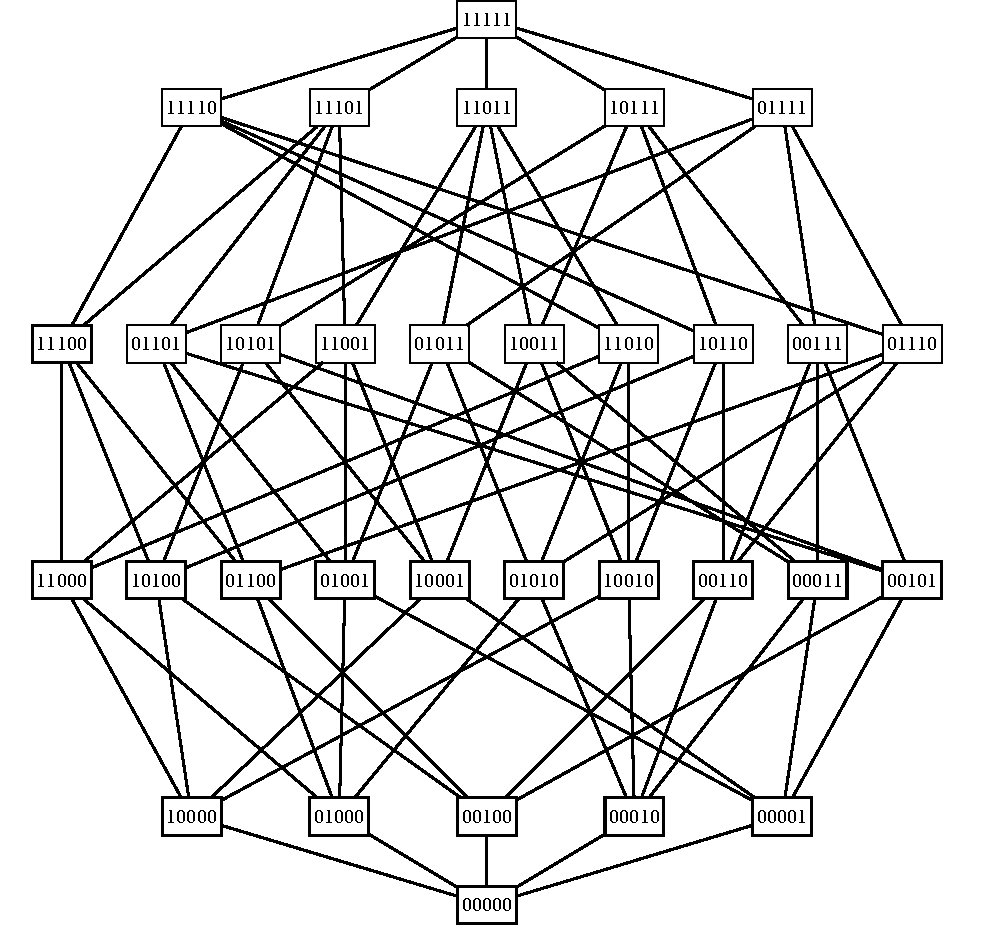
\includegraphics[clip=true]{pucs/partition/full_lattice.pdf}}
     \label{fig:pucs_part:full} }
    & 
    \subfigure[] {\scalebox{.75}{
    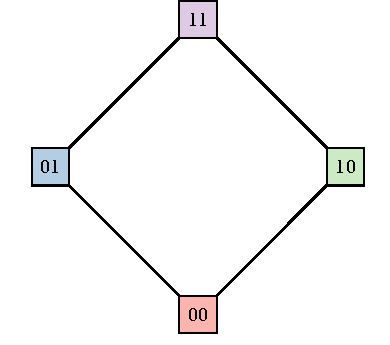
\includegraphics[clip=true]{pucs/partition/external_lattice.pdf}}
    \label{fig:pucs_part:external} }
    \\
    \subfigure[] {\scalebox{.8}{
    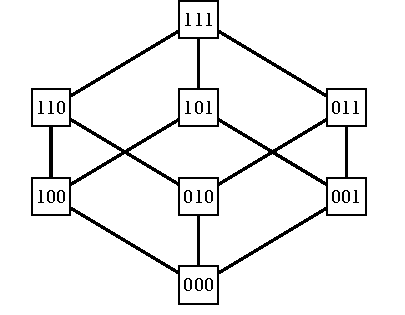
\includegraphics[clip=true]{pucs/partition/internal_lattice.pdf}}
    \label{fig:pucs_part:internal} }
    &
    \subfigure[] {\scalebox{0.3}{
    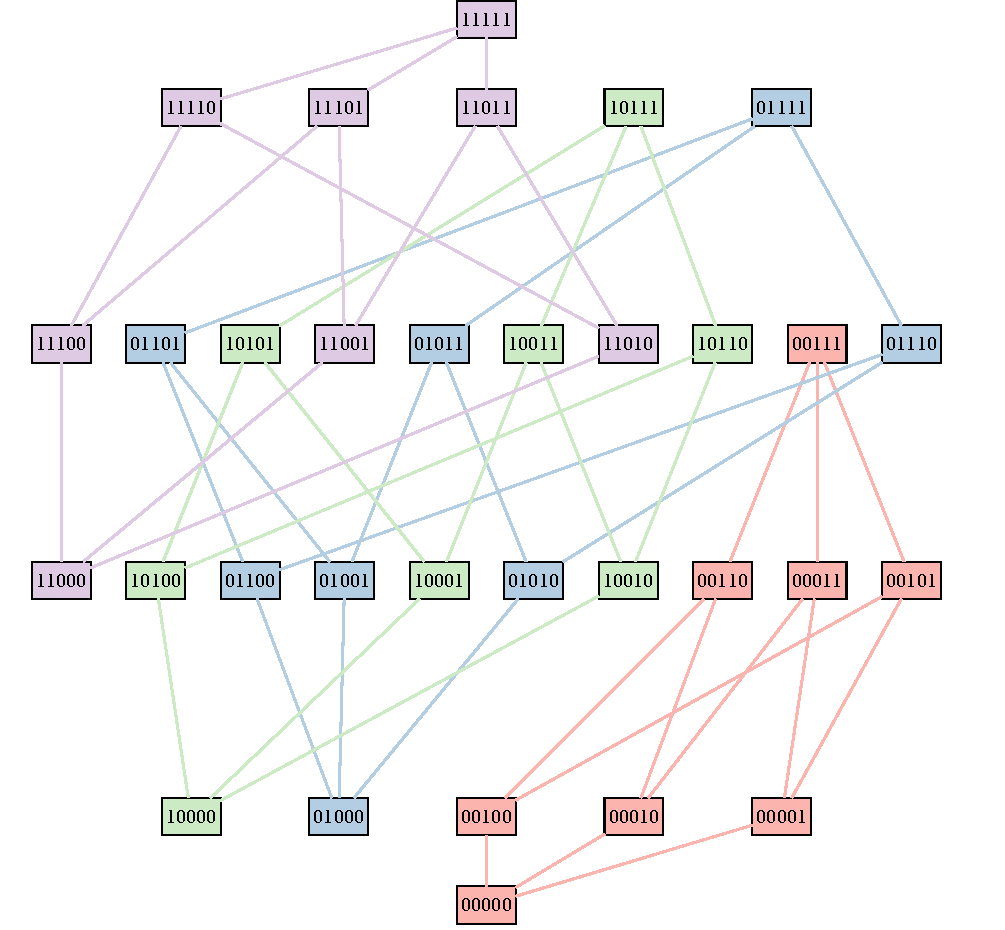
\includegraphics[clip=true]{pucs/partition/all_parts.pdf}}
    \label{fig:pucs_part:parts} }   
    \\
  \end{tabular}
    \caption{Exemplo de particionamento feito pelo algoritmo 
    \algname{PUCS} em uma instância com cinco características; o 
    reticulado Booleano desta instância é representado na figura~\ref{fig:pucs_part:full}. Neste particionamento, as duas primeiras
    variáveis formam o conjunto de variáveis fixadas, definindo o 
    reticulado externo (figura~\ref{fig:pucs_part:external}) enquanto 
    as outras três definem os reticulados internos, que são cópias do
    reticulado da figura~\ref{fig:pucs_part:internal}. A figura~\ref{fig:pucs_part:parts} mostra o reticulado Booleano original, sem
    as arestas que ligam duas partes diferentes, e a cor de cada nó 
    representa a qual parte tal nó pertence, de acordo com as cores
    do reticulado externo em~\ref{fig:pucs_part:external}
    Note que, de fato, 
    cada parte forma um reticulado pequeno de mesmo tamanho e com mesma 
    estrutura que o reticulado da figura~\ref{fig:pucs_part:internal}}.
  \label{fig:pucs_parts} 
\end{figure}

Dado o particionamento do espaço de busca e construção do reticulado 
externo, o algoritmo \algname{PUCS} descobre o mínimo global fazendo
um passeio pelo reticulado externo que deve armazenar partes candidatas
a conterem o mínimo global. O conjunto de partes candidatas a conter o
mínimo são resolvidas como problemas de seleção de características
auxiliares. Seja uma instância $\langle S, c \rangle$ do problema de
seleção de características, dado uma parte $P \in \powerset(S')$, 
o mínimo desta parte é o mínimo global do problema auxiliar 
$\langle \overline{S'}, c_P \rangle$, onde $c_P (X) = c (X \cup P)$.

Consideramos partes candidatas a conter o mínimo como aquelas que não
são podadas durante o passeio no reticulado externo. Antes de 
apresentar as condições de poda, definimos como ponta superior de um
reticulado $\powerset (A)$ como o conjunto $A$, e a ponta inferior como 
o conjunto $\emptyset$. Sejam $S$ um conjunto de características e $S'$ 
um conjunto de variáveis fixas no particionamento definido pelo 
algoritmo \algname{PUCS}; dados $P, Q \in \powerset (S')$ dois 
elementos do reticulado externo com $Q \subseteq P$, então as condições
de poda são:

\begin{itemize}
\item{se a ponta inferior do reticulado interno de $P$ tem custo maior 
do que a ponta inferior do reticulado interno de $Q$, então todas as 
partes do intervalo $[P, S']$ podem ser podadas, pois possuem 
reticulados internos cujos elementos terão custo maior do que o custo da 
ponta inferior do reticulado interno de $Q$.}
\item{se a ponta superior do reticulado interno de $P$ tem custo menor
do que a ponta superior do reticulado interno de $Q$, então todas as 
partes do intervalo $[\emptyset, Q]$ podem ser podadas, pois possuem 
reticulados internos cujos elementos terão custo maior do que o custo da 
ponta superior do reticulado interno de $P$.}
\end{itemize}

Em nossa implementação, a solução de partes candidatas a conterem o 
mínimo global foi feita de maneira paralela. Note que assim o trabalho
é melhor distribuído quando comparado ao \algname{UBB-PFS}, pois o 
tamanho das partes do \algname{PUCS} são iguais. O algoritmo que resolve
o problema auxiliar de achar o mínimo local de uma parte é um dos 
parâmetros do algoritmo e será discutido em seguida.

O algoritmo \algname{PUCS} possui três parâmetros de funcionamento. 
Chamamos de algoritmo base o parâmetro que define o algoritmo que será 
utilizado para se resolver cada parte candidata. O parâmetro $l$ define
quantas chamadas recursivas do \algname{PUCS} serão aplicadas nas 
soluções das partes antes que o algoritmo base seja chamado. Por último,
o parâmetro $p$ define a proporção de variáveis do problema que serão
fixadas no particionamento.

Observamos em nossos testes que quando o algoritmo base utilizado é
uma heurística, então os parâmetros $p$ e $l$ definem o tempo de 
execução e ao mesmo tempo a qualidade da solução obtida. Quanto maior
o valor destes parâmetros, mais próximo a resposta estará da solução 
ótima, entretanto, maior será o tempo de execução. A 
figura~\ref{fig:pucs:parameters:big} mostra para instâncias de 
duzentas características como os parâmetros $p$ e $l$ afetam a qualidade
da solução e o tempo de execução do \algname{PUCS} quando o algoritmo
base é a heurística \algname{Sequential Forward Floating Selection} 
(\algname{SFFS})~\cite{PNK94}.

\begin{figure}[!ht]
    \begin{center}
    \begin{tabular}{l r}
    \centering
        \subfigure[] {
        \label{fig:pucs:parameters:big:A}
        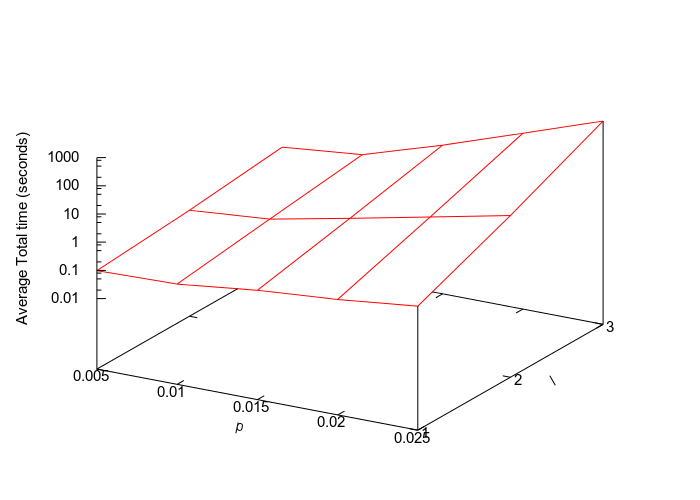
\includegraphics[clip=true, width=0.48\textwidth]{pucs/parameters/n200-20-3_time.png}
    }
    &
        \subfigure[] {
        \label{fig:pucs:parameters:big:B}
        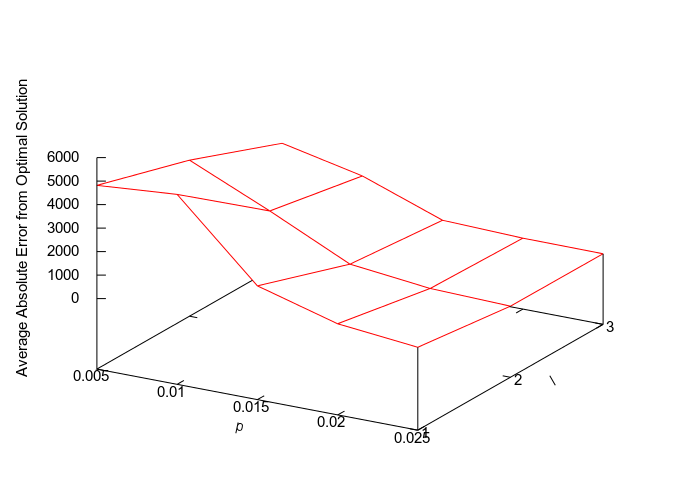
\includegraphics[clip=true, width=0.48\textwidth]{pucs/parameters/n200-20-3_error.png}
    }
    \end{tabular}   
    \end{center}
    \caption{Desempenho do algoritmo \algname{PUCS} para uma 
    instância artificial de 200 características utilizando o 
    \algname{SFFS} como algoritmo base e variando os parâmetros
    $p$ e $l$. A figura~\ref{fig:pucs:parameters:big:A} mostra o tempo
    médio de execução, note que este aumenta quando aumentamos os 
    parâmetros. A figura~\ref{fig:pucs:parameters:big:B} mostra a 
    diferença absoluta média entre o custo do conjunto obtido e do 
    conjunto ótimo.}
    \label{fig:pucs:parameters:big}
\end{figure}

Separamos os testes do \algname{PUCS} em testes ótimos, em que as 
instâncias tem tamanho pequeno o suficiente para poderem ser resolvidas
otimamente, e em testes sub-ótimos, em que o tamanho da instância é 
muito grande para ser resolvida otimamente. Nos testes ótimos, 
utilizamos como algoritmo base o \algname{UBB}, enquanto que nos testes 
sub-ótimos utilizamos a heurística \algname{SFFS}. Em ambos os testes
utilizamos valores de $p$ tal que o número de variáveis fixas é 10,
e $l = 1$. Estes valores de $p$ e $l$ foram escolhidos empiricamente 
como os melhores para a máquina utilizada para os testes.

Os resultados dos experimentos ótimos são apresentados nas
tabelas~\ref{tab:pucs:small:time}~e~\ref{tab:pucs:small:cost}, e nelas
podemos observar que o \algname{PUCS} teve desempenho similar ou pouco
pior do que \algname{UBB-PFS}. Já nos experimentos sub-ótimos, 
apresentados na figura~\ref{fig:pucs:big}, podemos observar que, apesar 
do \algname{PUCS} ter tempo de execução maior do que as outras 
heurísticas, \algname{SFFS} e \algname{Best\--First\--Search} 
(\algname{BFS}), a proporção de vezes em que o \algname{PUCS} encontrou 
a melhor solução entre os três algoritmos foi de $100\%$. Desta forma, 
podemos considerar o \algname{PUCS} como uma alternativa competitiva 
para instâncias grandes do problema U-curve.

\begin{table}
\centering
\footnotesize
\begin{tabular}{cc c cccc}
\toprule
\multicolumn{2}{c}{Instance} & \phantom{} & \multicolumn{4}{c}{Total time (sec)} \\
\cline{1-2}\cline{4-7}\\
$|S|$ & $2^{|S|}$ && \algname{UBB} & \algname{PFS} & \algname{UBB-PFS} & \algname{PUCS} \\
10 &    1024 &&  0.006 $\pm$ 0.001 & 0.011 $\pm$ 0.002 & 0.022 $\pm$ 0.004 & 0.039 $\pm$ 0.019 \\
11 &    2048 &&  0.007 $\pm$ 0.002 & 0.017 $\pm$ 0.004 & 0.026 $\pm$ 0.005 & 0.045 $\pm$ 0.022 \\
12 &    4096 &&  0.009 $\pm$ 0.003 & 0.029 $\pm$ 0.009 & 0.033 $\pm$ 0.008 & 0.048 $\pm$ 0.024 \\
13 &    8192 &&  0.013 $\pm$ 0.006 & 0.054 $\pm$ 0.016 & 0.047 $\pm$ 0.014 & 0.053 $\pm$ 0.021 \\
14 &   16384 &&  0.026 $\pm$ 0.012 & 0.103 $\pm$ 0.035 & 0.074 $\pm$ 0.017 & 0.057 $\pm$ 0.024 \\
15 &   32768 &&  0.048 $\pm$ 0.027 & 0.195 $\pm$ 0.080 & 0.116 $\pm$ 0.044 & 0.056 $\pm$ 0.025 \\
16 &   65536 &&  0.097 $\pm$ 0.055 & 0.354 $\pm$ 0.176 & 0.198 $\pm$ 0.089 & 0.090 $\pm$ 0.080 \\
17 &  131072 &&  0.142 $\pm$ 0.120 & 0.676 $\pm$ 0.375 & 0.350 $\pm$ 0.200 & 0.255 $\pm$ 0.276 \\
18 &  262144 &&  0.319 $\pm$ 0.228 & 1.512 $\pm$ 0.764 & 0.751 $\pm$ 0.338 & 0.680 $\pm$ 0.592 \\
19 &  524288 &&  0.684 $\pm$ 0.464 & 2.875 $\pm$ 1.554 & 1.387 $\pm$ 0.707 & 1.492 $\pm$ 1.323 \\
20 & 1048576 &&  1.249 $\pm$ 0.975 & 5.295 $\pm$ 3.509 & 2.594 $\pm$ 1.569 & 2.701 $\pm$ 2.908 \\
21 & 2097152 &&  2.671 $\pm$ 1.948 & 11.136 $\pm$ 6.947 & 5.460 $\pm$ 3.392 & 6.118 $\pm$ 5.961 \\
22 & 4194304 &&  5.420 $\pm$ 4.202 & 19.825 $\pm$ 14.519 & 9.709 $\pm$ 7.319 & 11.729 $\pm$ 11.613 \\
\bottomrule
\end{tabular}
\caption{Comparação de tempo de execução de algoritmos ótimos para o
problema U-curve. O \algname{PUCS} foi o segundo algoritmo mais lento,
sendo mais rápido do que o \algname{PFS} apenas.}
\label{tab:pucs:small:time}
\end{table}

\begin{table}
\centering
\footnotesize
\resizebox{\columnwidth}{!}{%
\begin{tabular}{cc c cccc}
\toprule
\multicolumn{2}{c}{Instance} & \phantom{} & \multicolumn{4}{c}{\# Calls of cost function} \\
\cline{1-2}\cline{4-7}\\
$|S|$ & $2^{|S|}$ && \algname{UBB} & \algname{PFS} & \algname{UBB-PFS} & \algname{PUCS} \\
 % 1 &       2 && 2.0 $\pm$  0.0 &  2.0 $\pm$  0.0 &  2.0 $\pm$  0.0 &  5.0 $\pm$  0.0 \\
 % 2 &       4 && 3.8 $\pm$  0.4 &  3.9 $\pm$  0.2 &  3.8 $\pm$  0.4 &  7.4 $\pm$  0.9 \\
 % 3 &       8 && 6.9 $\pm$  1.3 &  7.7 $\pm$  0.5 &  6.9 $\pm$  1.3 & 15.0 $\pm$  3.2 \\
 % 4 &      16 && 13.1 $\pm$  3.5 & 13.1 $\pm$  2.9 & 13.1 $\pm$  3.5 & 28.6 $\pm$  8.1 \\
 % 5 &      32 && 25.0 $\pm$  8.2 & 25.4 $\pm$  5.1 & 24.4 $\pm$  7.5 & 50.3 $\pm$ 14.4 \\
 % 6 &      64 && 50.7 $\pm$ 16.7 & 49.6 $\pm$ 13.9 & 49.3 $\pm$ 14.4 & 97.8 $\pm$ 32.9 \\
 % 7 &     128 && 101.6 $\pm$ 34.2 & 80.2 $\pm$ 29.3 & 95.1 $\pm$ 24.9 & 167.4 $\pm$ 57.6 \\
 % 8 &     256 && 166.2 $\pm$ 89.6 & 173.0 $\pm$ 33.9 & 162.7 $\pm$ 69.7 & 274.1 $\pm$ 136.8 \\
 % 9 &     512 && 356.2 $\pm$ 193.1 & 313.0 $\pm$ 91.9 & 323.1 $\pm$ 126.6 & 472.8 $\pm$ 285.4 \\
10 &    1024 && 668.2 $\pm$ 359.2 & 614.2 $\pm$ 162.7 & 630.3 $\pm$ 235.9 & 753.6 $\pm$ 493.6 \\
11 &    2048 && 1171.5 $\pm$ 742.5 & 1139.2 $\pm$ 354.0 & 1174.8 $\pm$ 499.3 & 1305.0 $\pm$ 881.8 \\
12 &    4096 && 2611.6 $\pm$ 1528.5 & 2137.1 $\pm$ 793.3 & 2271.2 $\pm$ 894.1 & 2370.5 $\pm$ 1615.7 \\
13 &    8192 && 4583.2 $\pm$ 2910.2 & 4218.9 $\pm$ 1306.7 & 4308.7 $\pm$ 1732.2 & 4780.0 $\pm$ 2797.7 \\
14 &   16384 && 10781.4 $\pm$ 5565.5 & 8211.1 $\pm$ 3054.5 & 9050.4 $\pm$ 2638.1 & 7050.8 $\pm$ 4755.7 \\
15 &   32768 && 20891.9 $\pm$ 12757.0 & 15134.0 $\pm$ 6528.5 & 15900.7 $\pm$ 6927.4 & 14080.1 $\pm$ 11373.1 \\
16 &   65536 && 43529.6 $\pm$ 25318.9 & 26447.0 $\pm$ 13446.1 & 28783.6 $\pm$ 12934.2 & 26001.3 $\pm$ 21699.6 \\
17 &  131072 && 65301.0 $\pm$ 56215.8 & 49694.5 $\pm$ 27621.8 & 51032.5 $\pm$ 29984.3 & 50145.2 $\pm$ 46799.0 \\
18 &  262144 && 145594.5 $\pm$ 103597.8 & 105603.1 $\pm$ 52652.2 & 110538.0 $\pm$ 51589.7 & 111296.6 $\pm$ 84922.4 \\
19 &  524288 && 313096.0 $\pm$ 209913.1 & 194572.5 $\pm$ 104802.3 & 204604.5 $\pm$ 100305.4 & 233717.7 $\pm$ 186182.0 \\
20 & 1048576 && 578319.0 $\pm$ 445912.2 & 340052.5 $\pm$ 221271.6 & 362007.0 $\pm$ 207411.2 & 387082.0 $\pm$ 389417.4 \\
% 21 & 2097152 && 1208939.1 $\pm$ 867260.3 & 699906.1 $\pm$ 437209.1 & 726193.9 $\pm$ 420497.8 & 854293.9 $\pm$ 779635.6 \\
% 22 & 4194304 && 2375634.9 $\pm$ 1826536.5 & 1195439.1 $\pm$ 881956.5 & 1253704.3 $\pm$ 847533.7 & 1640138.3 $\pm$ 1547703.6 \\
\bottomrule
\end{tabular}
}
\caption{Comparação de número de chamadas da função custo em algoritmos
ótimos do problema U-curve. O \algname{PUCS} faz menos chamadas da
função custo que o \algname{UBB}, porém faz mais chamadas do que o 
\algname{PFS} e \algname{UBB-PFS}.}
\label{tab:pucs:small:cost}
\end{table}


\begin{figure}[!ht]
    \begin{center}
    \begin{tabular}{l r}
    \centering
        \subfigure[] {
        \label{fig:pucs:big:time}
        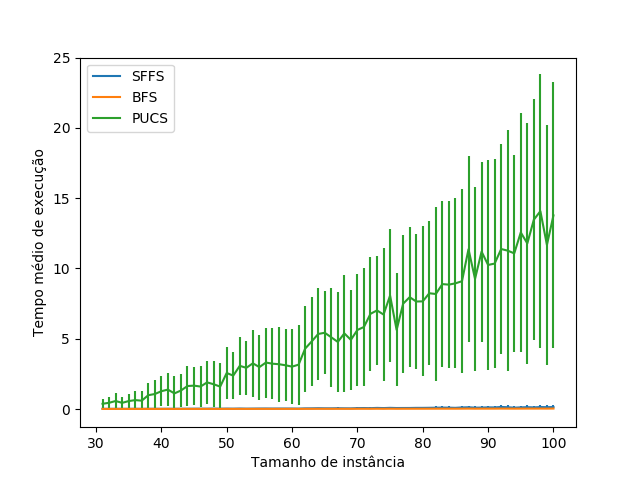
\includegraphics[clip=true, width=0.5\textwidth]{pucs/experiments/time_sffs_bfs_pucs.png}
    }
    &
        \subfigure[] {
        \label{fig:pucs:big:correctness}
        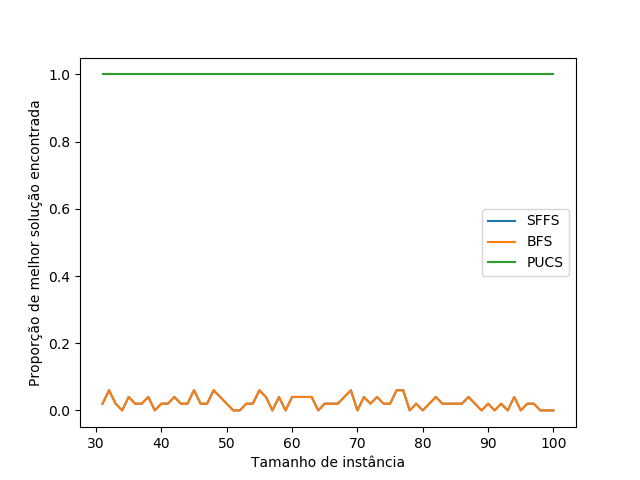
\includegraphics[clip=true, width=0.5\textwidth]{pucs/experiments/correctness_sffs_bfs_pucs.png}
    }
    \end{tabular}   
    \end{center}
    \caption{Comparação entre os algoritmos \algname{SFFS}, 
    \algname{BFS} e \algname{PUCS}. A figura~\ref{fig:pucs:big:time} 
    mostra o tempo médio de execução dos algoritmos. A 
    figura~\ref{fig:pucs:big:correctness} mostra a proporção de vezes
    em que cada algoritmo achou a melhor resposta entre os três.}
    \label{fig:pucs:big}
\end{figure}


\subsection{Testes com instâncias reais do problema de seleção de 
            características}
Como última atividade deste projeto, investigamos o uso de seleção de
características na seleção de modelos de aprendizado. Com conjuntos de 
dados do
\href{https://archive.ics.uci.edu/ml/index.php}{University of California Irvine (UCI) Machine Learning Repository}~\cite{Lic13}, criamos modelos com e sem seleção de características e
avaliamos os erros médios de seus classificadores. Foi empregado o 
algoritmo \algname{PUCS} para esta seleção.

Em ambos modelos (com e sem seleção de características) definimos 
classificadores do tipo Support Vector Machine (SVM), com kernel linear.
Como parâmetro $C$ de regularização, utilizamos o valor $100$, que é 
propositalmente alto, pois queremos observar a regularização vinda da 
própria seleção de características. O erro de ambos modelos foi estimado 
com o esquema de validação cruzada; para conjuntos de dados com mais de 
100 amostras, utiliza-se validação cruzada 10-\foreignword{fold}, caso 
contrário, utiliza-se a validação \foreignword{leave-one-out}.

A figura~\ref{fig:uci} mostra os resultados deste teste. Podemos 
observar que o número médio de características selecionadas é 
significativamente menor para a maioria destes conjuntos de dados; no 
conjunto Promoters, por exemplo, menos de 10 características são 
selecionadas em um total de 57. Esta diminuição implica na diminuição
da complexidade do modelo, o que é benéfico em aprendizado de máquina 
tanto para efeito de tempo de execução quanto para o número de amostras 
requeridas para treinamento de um classificador que generaliza bem
um conjunto de dados. Além disso, a figura~\ref{fig:uci:error} mostra 
que mesmo com a simplificação do modelo feita pela seleção de 
características, a qualidade dos classificares não é significativamente
afetada; inclusive, para o conjunto de dados Lung Cancer, o erro médio 
dos classificadores diminui quando existe seleção de características.

\begin{figure}[!ht]
    \begin{center}
    \begin{tabular}{l r}
    \centering
        \subfigure[] {
        \label{fig:uci:feats}
        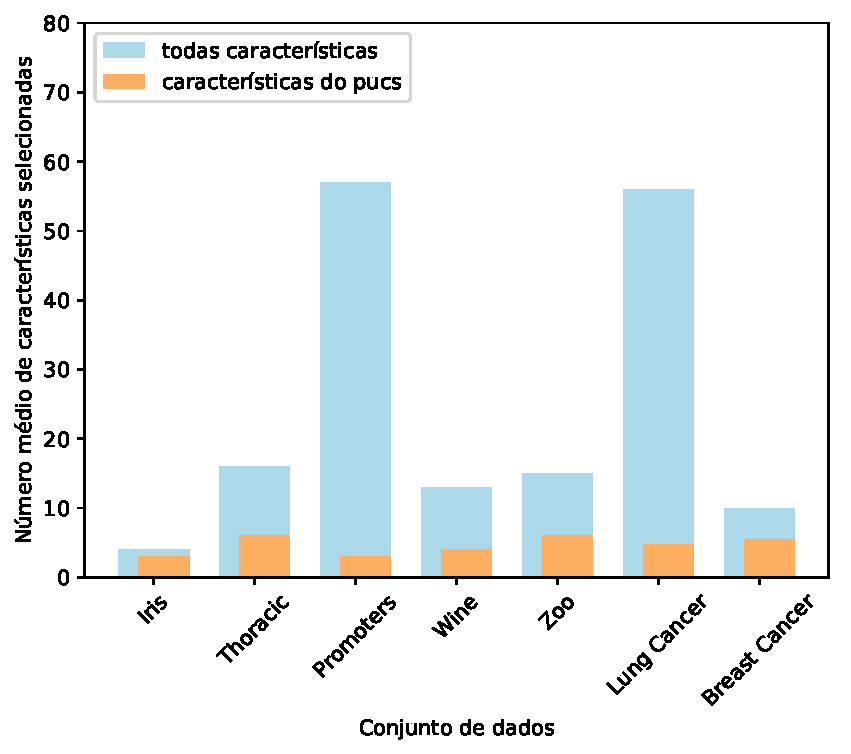
\includegraphics[clip=true, width=0.45\textwidth]{uci/avg_features.pdf}
    }
    &
        \subfigure[] {
        \label{fig:uci:error}
        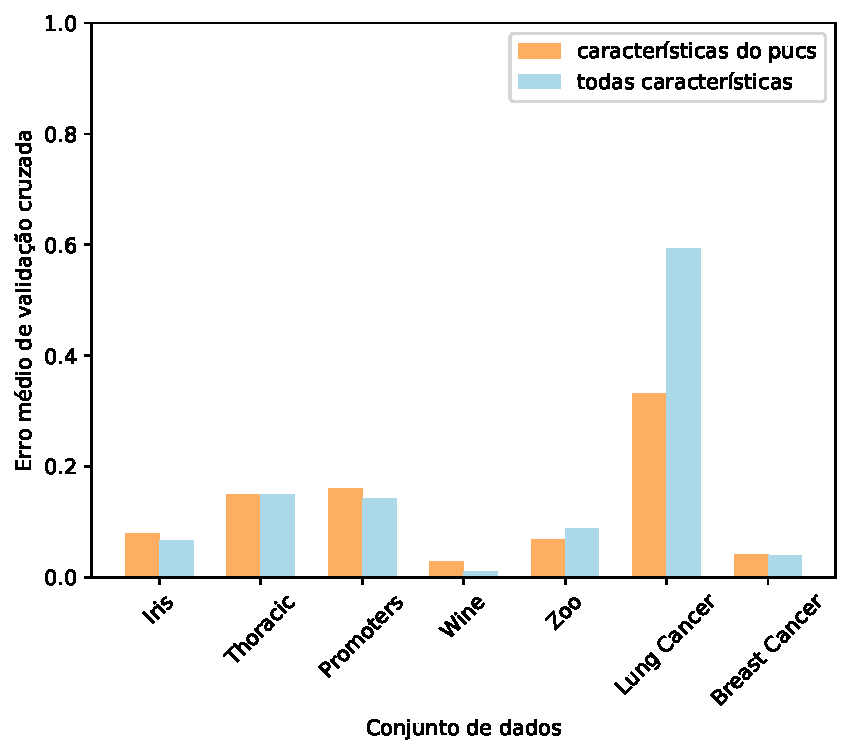
\includegraphics[clip=true, width=0.45\textwidth]{uci/svm_error.pdf}
    }
    \end{tabular}   
    \end{center}
    \caption{Comparações de modelos feitos com todas características e
        com a características selecionadas pelo \algname{PUCS}. A 
        figura~\ref{fig:uci:feats} mostra a quantidade de 
        atributos selecionados pelo algoritmo em cada conjunto
        de dados, enquanto a figura~\ref{fig:uci:error} mostra o erro
        de validação cruzada dos modelos feitos com todas 
        características e apenas com as características selecionadas.}
    \label{fig:uci}
\end{figure}


\section{Avaliação e disseminação de resultados}
\subsection{Participação em conferências}
% - x-meeting
% - rca
% -> apresentação de poster

\subsection{Monografia de conclusão de curso}
% - mencionar que tirou 10

\subsection{Publicações}
% com os esforços desta ic e da última:
% - paper featsel publicado
% - paper UCS em revisão
% - paper PUCS em preparação

\section{Conclusão} 
% - balanço do trabalho 
% - como acreditamos que este trabalho impacta no trabalho de mestrado
\pagebreak


\begin{thebibliography}{9} \label{sec:referencias}

\addcontentsline{toc}{section}{Referências}

\bibitem{msreis thesis}
Reis, Marcelo S. ``Minimization of decomposable in U-shaped curves functions defined on poset chains–algorithms and applications." PhD thesis, Institute of Mathematics and Statistics, University of São Paulo, Brazil, (2012).

\bibitem{featsel paper}
Reis, Marcelo S., Gustavo Estrela, Carlos E. Ferreira e Junior Barrera.
``featsel: A framework for benchmarking of feature selection algorithms
and cost functions". SoftwareX 6 (2017), pp. 193-197.

\bibitem{bryant}
Bryant, Randal E. ``Graph-based algorithms for boolean function manipulation." IEEE Transactions on Computers, 100.8 (1986): 677-691. 

\bibitem{ic1}
Gustavo E. Matos e Marcelo S. Reis. ``Estudos de estruturas de dados 
eficientes para abordar o problema de otimização U-curve". Relatório
científico final FAPESP, Instituto Butantan, Brasil (2015).

\bibitem{PNK94}
P. Pudil, J. Novovičová, e J. Kittler. ``Floating search methods in feature selection". 
Pattern Recognition Letters 15.11 (1994), pp. 1119-1125.


\bibitem{Lic13}
M. Lichman. UCI Machine Learning Repository. 2013. 
URL:https://archive.ics.uci.edu/ml.

\end{thebibliography}

\end{document}


